%  -----------------------------------------------------------------------------
%  Author         : Bimalka Piyaruwan Thalagala
%  GitHub         : https://github.com/bimalka98
%  Date Created   : 01.09.2020
%  Last Modified  : 06.03.2020
%  -----------------------------------------------------------------------------

\documentclass[a4paper,11pt]{article}%,twocolumn
%% packages


\usepackage{amsmath} % needed for command eqref
\usepackage{amssymb} % needed for math fonts
\usepackage[colorlinks=true,breaklinks]{hyperref} % needed for creating hyperlinks in the document, the option colorlinks=true gets rid of the awful boxes, breaklinks breaks lonkg links (list of figures), and ngerman sets everything for german as default hyperlinks language
\usepackage[hyphenbreaks]{breakurl} % ben�tigt f�r das Brechen von URLs in Literaturreferenzen, hyphenbreaks auch bei links, die �ber eine Seite gehen (mit hyphenation).
\usepackage{xcolor}
\definecolor{c1}{rgb}{0,0,1} % blue
\definecolor{c2}{rgb}{0,0.3,0.9} % light blue
\definecolor{c3}{rgb}{0.3,0,0.9} % red blue
\hypersetup{
    linkcolor={c1}, % internal links
    citecolor={c2}, % citations
    urlcolor={c3} % external links/urls
}
%\usepackage{cite} % needed for cite
\usepackage[square,authoryear]{natbib} % needed for cite and abbrvnat bibliography style
\usepackage[nottoc]{tocbibind} % needed for displaying bibliography and other in the table of contents
\usepackage{graphicx} % needed for \includegraphics 
\usepackage{longtable} % needed for long tables over pages
\usepackage{bigstrut} % needed for the command \bigstrut
\usepackage{enumerate} % needed for some options in enumerate
%\usepackage{todonotes} % needed for todos
\usepackage{makeidx} % needed for creating an index
\makeindex
\usepackage{gensymb}
\usepackage{url}
\usepackage{psfrag}
\usepackage{multirow}
\usepackage{subfigure}
\usepackage{epstopdf}

%% page settings

\usepackage[top=20mm, bottom=20mm,left=15mm,right=15mm]{geometry} % needed for page border settings
\parindent=0mm % for space of first line of new text block
\sloppy % for writing with hyphenless justification (tries to)
\hyphenation{} % use hyphenation of tolerance parametershttp://www.jr-x.de/publikationen/latex/tipps/zeilenumbruch.html
\hyphenpenalty=10000
\exhyphenpenalty=10000
\usepackage{fancyhdr} % needed for head and foot options
%% my macros

%% Text fomats
\newcommand{\tbi}[1]{\textbf{\textit{#1}}}

%% Math fonts
\newcommand{\bbA}{\mathbb{A}}
\newcommand{\bbB}{\mathbb{B}}
\newcommand{\bbC}{\mathbb{C}}
\newcommand{\bbD}{\mathbb{D}}
\newcommand{\bbE}{\mathbb{E}}
\newcommand{\bbF}{\mathbb{F}}
\newcommand{\bbG}{\mathbb{G}}
\newcommand{\bbH}{\mathbb{H}}
\newcommand{\bbI}{\mathbb{I}}
\newcommand{\bbJ}{\mathbb{J}}
\newcommand{\bbK}{\mathbb{K}}
\newcommand{\bbL}{\mathbb{L}}
\newcommand{\bbM}{\mathbb{M}}
\newcommand{\bbN}{\mathbb{N}}
\newcommand{\bbO}{\mathbb{O}}
\newcommand{\bbP}{\mathbb{P}}
\newcommand{\bbQ}{\mathbb{Q}}
\newcommand{\bbR}{\mathbb{R}}
\newcommand{\bbS}{\mathbb{S}}
\newcommand{\bbT}{\mathbb{T}}
\newcommand{\bbU}{\mathbb{U}}
\newcommand{\bbV}{\mathbb{V}}
\newcommand{\bbW}{\mathbb{W}}
\newcommand{\bbX}{\mathbb{X}}
\newcommand{\bbY}{\mathbb{Y}}
\newcommand{\bbZ}{\mathbb{Z}}
\usepackage[ framed, numbered]{matlab-prettifier}%framed,%
\usepackage{listings}
\usepackage{physics}
\usepackage{pdfpages}
\usepackage[toc,page]{appendix}

\begin{document}
\begin{titlepage}
\center % Center everything on the page

%-------------------------------------------------------------------------------------
%	HEADING SECTIONS
%------------------------------------------------------------------------------------
\textbf{\large Department of Electronic and Telecommunication Engineering}\\[0.5cm]
\textbf{\Large University of Moratuwa, Sri Lanka}\\[1cm]
\textbf{\large EN2570 - Digital Signal Processing}\\[2cm]

\includegraphics[width=0.3\textwidth]{figures/uomlogo}\\[2cm]

	
%-------------------------------------------------------------------------------------
%	TITLE SECTION
%------------------------------------------------------------------------------------
\textbf{\Huge Design of an FIR Digital Filter for Prescribed Specifications}\\[0.2cm]
{\Large (Using the windowing method in conjunction with the Kaiser window)}\\[0.5cm]
\textbf{\Large Project Report}\\[5cm]


%----------------------------------------------------------------------------------------
%	MEMBERS SECTION
%----------------------------------------------------------------------------------------

\vfill
\textbf{\large Submitted by}\\[0.5cm]
\begin{minipage}{0.2\textwidth}
	\begin{flushleft}
		{\large Thalagala B.P.}\\[4mm]		
	\end{flushleft}
\end{minipage}
\hspace{2mm}
\begin{minipage}{0.2\textwidth}
	\begin{flushright}
		{\large 180631J }\\[4mm]
	\end{flushright}
\end{minipage}\\[1.5cm]

%----------------------------------------------------------------------------------------
%	DATE SECTION
%----------------------------------------------------------------------------------------

\textbf{\large Submitted on}\\[0.5cm]
\textbf{\Large \today} % Date, change the \today to a set date if you want to be precise

%----------------------------------------------------------------------------------------

\vfill % Fill the rest of the page with whitespace

\end{titlepage}

\begin{abstract}
	Design procedure of a Finite Duration Impulse Response(FIR) bandpass Digital Filter which satisfies a set of prescribed specifications, is described in this report where windowing method in conjunction with the Kaiser window is used for the designing procedure. Operation of the filter was analyzed with a combination of sinusoidal signals. The design was implemented and tested using {\tt MATLAB R2018a} of the MathWorks Inc.
\end{abstract}

\pagebreak

\tableofcontents
\listoffigures
\listoftables
\vfill
\begin{center}
	\textbf{\textit{*PDF is clickable}}
\end{center}

\textit{\textbf{Note:}}\\
\textit{All the materials and executable {\tt MATLAB R2018a} Live Script related to the project can also be found at \url{https://github.com/bimalka98/Digital-Signal-Processing}}
\pagebreak

\section{Introduction}

This report describes the design procedure of an FIR bandpass digital filter which satisfies a predefined set of specifications as shown in the Table \ref{filterspecs}.\textbf{\textit{ Kaiser windowing}} method is used, due to its excellent capability to control filter's ripple ratio  and main-lobe width to facilitate a given set of specification by simply varying the related parameters. And most importantly a method is available to calculate those parameters through empirical formulae. Therefore this Kaiser Window is heavily used to design filters with prescribed specifications.\\

{\tt MATLAB R2018a} of the MathWorks Inc. is used to implement and analyze the digital filter. Filtering was done in the frequency domain rather than in the time domain since the time domain convolution is computationally expensive. Frequency domain analysis was done using \textbf{\textit{Fast Fourier Transform}} algorithms(\textit{using built-in {\tt fft()} and {\tt ifft()} functions}). Performance of the filter was analyzed using a combination of sinusoidal signal, whose frequency components lie in the middle of the three main regions(\textit{lower stopband, passband and upper stopband}) of the bandpass filter. 

\section{Method}

First the digital filter is implemented through the procedure described in the \textbf{section 2.1}. Then its performance is analyzed as described in the \textbf{section 2.2}.

\subsection{Filter Implementation}
Digital filter implementation consists of the steps that are mentioned below. Subsections of this section of the report describes each one of them thoroughly for designing the FIR bandpass filter using Kaiser Window method.

\begin{enumerate}[\hspace{1cm}1.]
	\item Identifying the prescribed filter specifications
	\item Derivation of the filter Parameters
	\item Derivation of the Kaiser Window Parameters
	\item Derivation of The Ideal Impulse Response
	\item Truncating the Ideal Impulse Response to obtain Finite Impulse Response i.e Windowing
\end{enumerate}

\subsubsection{Prescribed Filter specifications}
Following table describes the desired specifications of the bandpass filter which need to be implemented. The notation used here is the same as the notation used in the reference material\cite{antonio} and they will be used throughout the report rather than numerical values.

\begin{table}[!h]
	\centering

	\begin{tabular}{l c r}
		\hline
		\textbf{Parameter}& \textbf{Symbol}&\textbf{Value}\\\hline
		&&\\
Maximum passband ripple(\textit{desired})&$\tilde{A_p}$&0.09 dB\\
Minimum stopband attenuation(\textit{desired})&$\tilde{A_a}$&48 dB\\
Lower passband edge&$\omega_{p1}$&400 rad/s\\
Upper passband edge&$\omega_{p2}$&800 rad/s\\
Lower stopband edge&$\omega_{a1}$&250 rad/s\\
Upper stopband edge&$\omega_{a2}$&900 rad/s\\
Sampling frequency&$\omega_s$&2600 rad/s\\
\hline\hline
	\end{tabular}
	\caption{Prescribed Filter specifications}
	\label{filterspecs}
\end{table}

Following Fig.\ref{idealbpfilter} illustrates the aforementioned specifications graphically for an idealized frequency response of a Bandpass filter. $\delta$ in the figure has the following relationship with peak to peak passband ripple(\textit{practical}) $A_p$ and the minimum stopband attenuation(\textit{practical}) $A_a$.\\

\begin{equation}
	\tilde{A_p} \ge A_p = 20\log(\frac{1+\delta}{1-\delta})
	\label{A_p}
\end{equation}
\begin{equation}
 \tilde{A_a} \le A_a = -20\log(\delta)
 \label{A_a}
\end{equation}

\begin{figure}[!h]
	\centering
	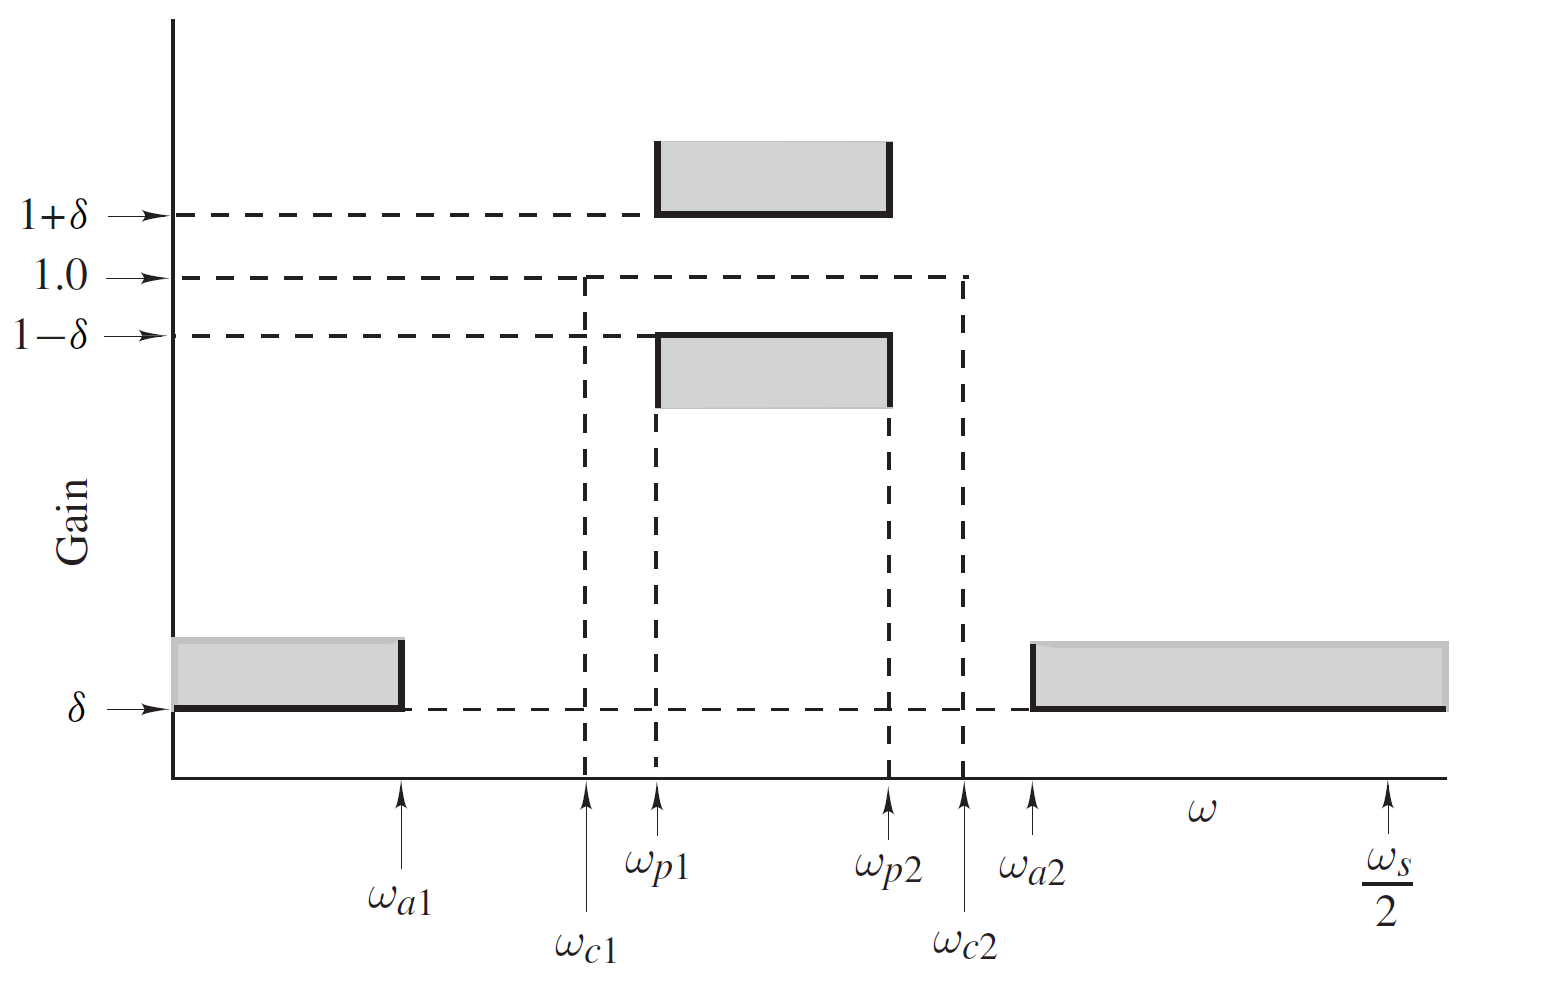
\includegraphics[scale=0.4]{figures/filtersepecs}
	\caption{Idealized frequency response of a Bandpass filter\cite{antonio}}
	\label{idealbpfilter}
\end{figure}

\subsubsection{Derivation of filter Parameters}

According to the given specifications following parameters are calculated; which then will be used to derive the parameters of the Kaiser window.  

\begin{table}[!h]
	\centering	
\begin{tabular}{l c c r}
	\hline
\textbf{Parameter}& \textbf{Symbol}& \textbf{Calculation}&\textbf{Value}\\\hline
&&&\\
Lower transition width& $B_{t1}$& $\omega_{p1} - \omega_{a1}$&150 rad/s\\
Upper transition width& $B_{t2}$&$\omega_{a2}-\omega_{p2}$&100 rad/s\\
Critical transition width& $B_t$&$\min(B_{t1},B_{t2})$&100 rad/s\\
Lower cutoff frequency& $\omega_{c1}$&$\omega_{p1}-B_t/2$&350 rad/s\\
Upper cutoff frequency& $\omega_{c2}$&$\omega_{p2}+B_t/2 $&850 rad/s \\
Sampling period& $T$& $2\pi / \omega_s$&$0.0024$ s\\
\hline\hline
\end{tabular}
\caption{Derivation of filter Parameters}
\end{table}

\subsubsection{Derivation of the Kaiser Window Parameters}

Following equation represents the Kaiser window which will be used to truncate the Infinite duration Impulse Response to obtain the Finite duration Impulse Response for our filter design. Further explanations of the same steps can be found in the \textit{sections 9.4.5} and \textit{9.4.6} in the reference material\cite{antonio}.

\begin{equation}
w_K(nT) = \begin{cases}
	\frac{I_0(\beta)}{I_0(\alpha)} & for \abs{n}  \leq \frac{N-1}{2} \\
	0 & Otherwise
	\label{kaiser}
\end{cases}
\end{equation}


where $\alpha$ is an independent parameter and $I_0(x)$ is the zeroth-order modified Bessel function of the first kind.\\
%372
\[
\beta = \alpha\sqrt{1-\left(\frac{2n}{N-1}\right)^2} \hspace*{1cm} \hspace*{1cm} I_0(x) = 1+\sum_{k=1}^{\infty}\left[\frac{1}{k!}\left(\frac{x}{2}\right)^k\right]^2
 \]

Now we have to calculate the required parameters as follows,

\begin{enumerate}[\hspace{1cm}a.)]
\item Choose $\delta$ in Eqs. \eqref{A_p} and \eqref{A_a} such that $\delta = \min(\tilde{\delta_p}, \tilde{\delta_a})$ where,

\[
\begin{split}
	\tilde{\delta_p} &= \frac{10^{0.05\tilde{A_p}}-1}{10^{0.05\tilde{A_p}}+1}\\
	&=\frac{10^{0.05*0.09}-1}{10^{0.05*0.09}+1}\\
	&=5.181\times10^{-3}
\end{split}
\hspace{2cm}
\begin{split}
	\tilde{\delta_a} &= 10^{-0.05\tilde{A_a}}\\
&=3.981\times10^{-3}
\end{split}
\]
\begin{center}
	$\therefore~ \delta = 3.981\times10^{-3} $
\end{center}

\item With the required $\delta$ defined, the actual stopband loss(attenuation) $A_a$ in dB can be calculated using Eq. \ref{A_a}.
\[
\begin{split}
	 \tilde{A_a} \le A_a &= -20\log(\delta)\\
	 &=-20\log(3.981\times10^{-3})\\
	A_a &= 48 ~dB
\end{split}
\]

\item Choose parameter $\alpha$ as,
    \[
\alpha = \begin{cases}
	0 & for~  A_a \leq 21 ~dB \\
	0.5842(A_a - 21)^{0.4} + 0.07886(A_a - 21) & for ~ 21 < A_a \leq 50 ~dB \\
	0.1102(A_a - 8.7) & for~  A_a > 50 ~dB
\end{cases}
\]

\[
\begin{split}
\therefore~ \alpha &= 0.5842(A_a - 21)^{0.4} + 0.07886(A_a - 21)\\
&=	0.5842(48 - 21)^{0.4} + 0.07886(48 - 21)\\
&=4.3125
\end{split}
\]

\item Choose parameter D as,

\[
D = \begin{cases}
	0.9222 & for ~ A_a \leq 21 ~dB \\

	\frac{A_a - 7.95}{14.36} & for ~ A_a > 21 ~dB
\end{cases}
\]\hspace{2cm}
\[
\begin{split}
	\therefore~ D &= \frac{A_a - 7.95}{14.36}\\
	&=\frac{48 - 7.95}{14.36}\\
	&=  2.7890
\end{split}
\]

\item Then select the lowest odd value of N that would satisfy the inequality,
\[
\begin{split}
	N  & \geq \frac{\omega_sD}{B_t}+1\\
	&\geq \frac{2600*2.79}{100}+1\\
	&\geq 73.51
\end{split}
\hspace{2cm}
\therefore~	N = 75
\]
\end{enumerate}

\begin{figure}[!h]
	\centering
	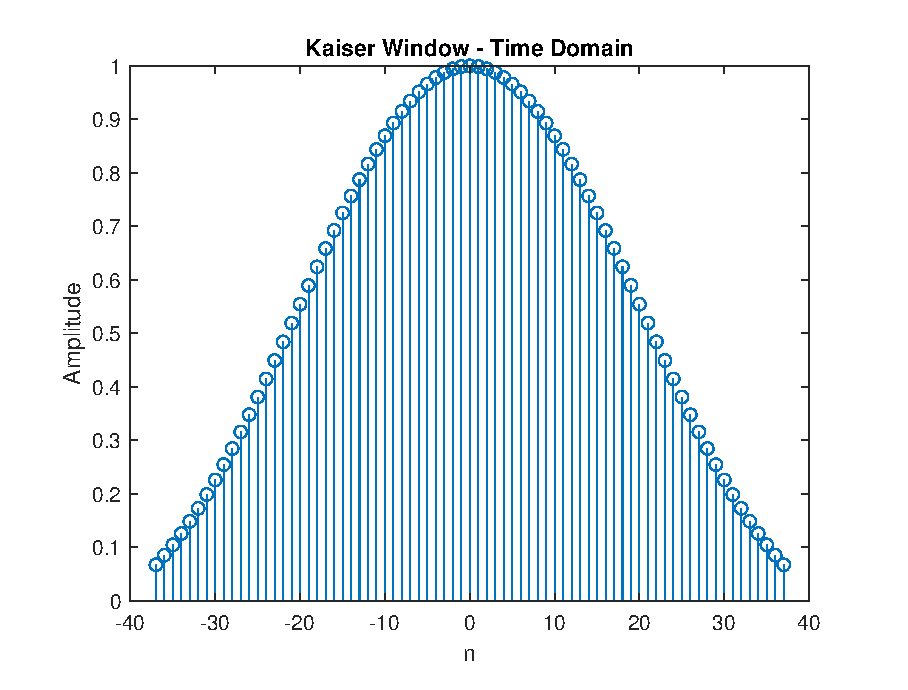
\includegraphics[scale=0.4]{figures/kaisertime}
	\caption{Derived Kaiser Window $w_K(nT)$ using calculated Parameters and Eq. \eqref{kaiser}}
\end{figure}

\subsubsection{Derivation of The Ideal Impulse Response}

\textbf{\textit{Note : Here subscript `d' implies ``desired'', as it is the ideal response of the filter. Subscript d will be omitted to indicate a given expression is no longer ideal.\\}}

The frequency response of an ideal bandpass filter with cutoff frequencies $\omega_{c1}$ and $\omega_{c2}$ is given by,

\[
H_d(e^{j\omega T}) = \begin{cases}
1& for~ -\omega_{c2} \le \omega \le -\omega_{c1}\\
1& for ~~~~~\omega_{c1} \le \omega \le \omega_{c2}\\
0& Otherwise
\end{cases}
\]

Using the Inverse Fourier Transform, impulse response of the above $H(e^{j\omega T})$ is calculated.
\[
\begin{split}
	h_d(nT) &=\frac{1}{\omega_s}\int_{-\omega_s/2}^{\omega_s/2} H(e^{j\omega T})e^{j\omega nT}~d\omega\\
	&=\frac{1}{\omega_s}\left[\int_{-\omega_{c2}}^{-\omega_{c1}} e^{j\omega nT} ~d\omega+ \int_{\omega_{c1}}^{\omega_{c2}} e^{j\omega nT}~ d\omega\right]\\
	&=\frac{1}{\omega_s} \left[ \left.\frac{e^{j\omega nT}}{jn T}\right|_{-\omega_{c2}}^{-\omega_{c1}} + \left.\frac{e^{j\omega nT}}{jn T}\right|_{\omega_{c1}}^{\omega_{c2}} \right]\\
	&= \frac{1}{j\omega_s nT} \left[  e^{-j\omega_{c1}nT} - e^{-j\omega_{c2}nT}  +  e^{j\omega_{c2}nT} - e^{j\omega_{c1}nT}  \right] ; where~\omega_sT = 2\pi\\
	&= \frac{1}{\pi n}\left[ \frac{(e^{j\omega_{c2}nT} - e^{-j\omega_{c2}nT})}{2j} - \frac{(e^{j\omega_{c1}nT} - e^{-j\omega_{c1}nT})}{2j}  \right] ; rearanging\\
	&=	\frac{1}{\pi n}\left[   \sin(\omega_{c2}nT) - \sin(\omega_{c1}nT)  \right]; from~ Euler's ~Eq.
\end{split}
\]

\begin{equation}
	\therefore ~ h_d(nT) = \begin{cases}
		\frac{1}{\pi n}\left[   \sin(\omega_{c2}nT) - \sin(\omega_{c1}nT)  \right] & \forall n \ne 0\\
		&\\
		\frac{2}{\omega_s}\left( \omega_{c2} - \omega_{c1}\right)& for~ n = 0
	\end{cases}
\label{idealresponse}
\end{equation}

\begin{figure}[!h]
	\centering
	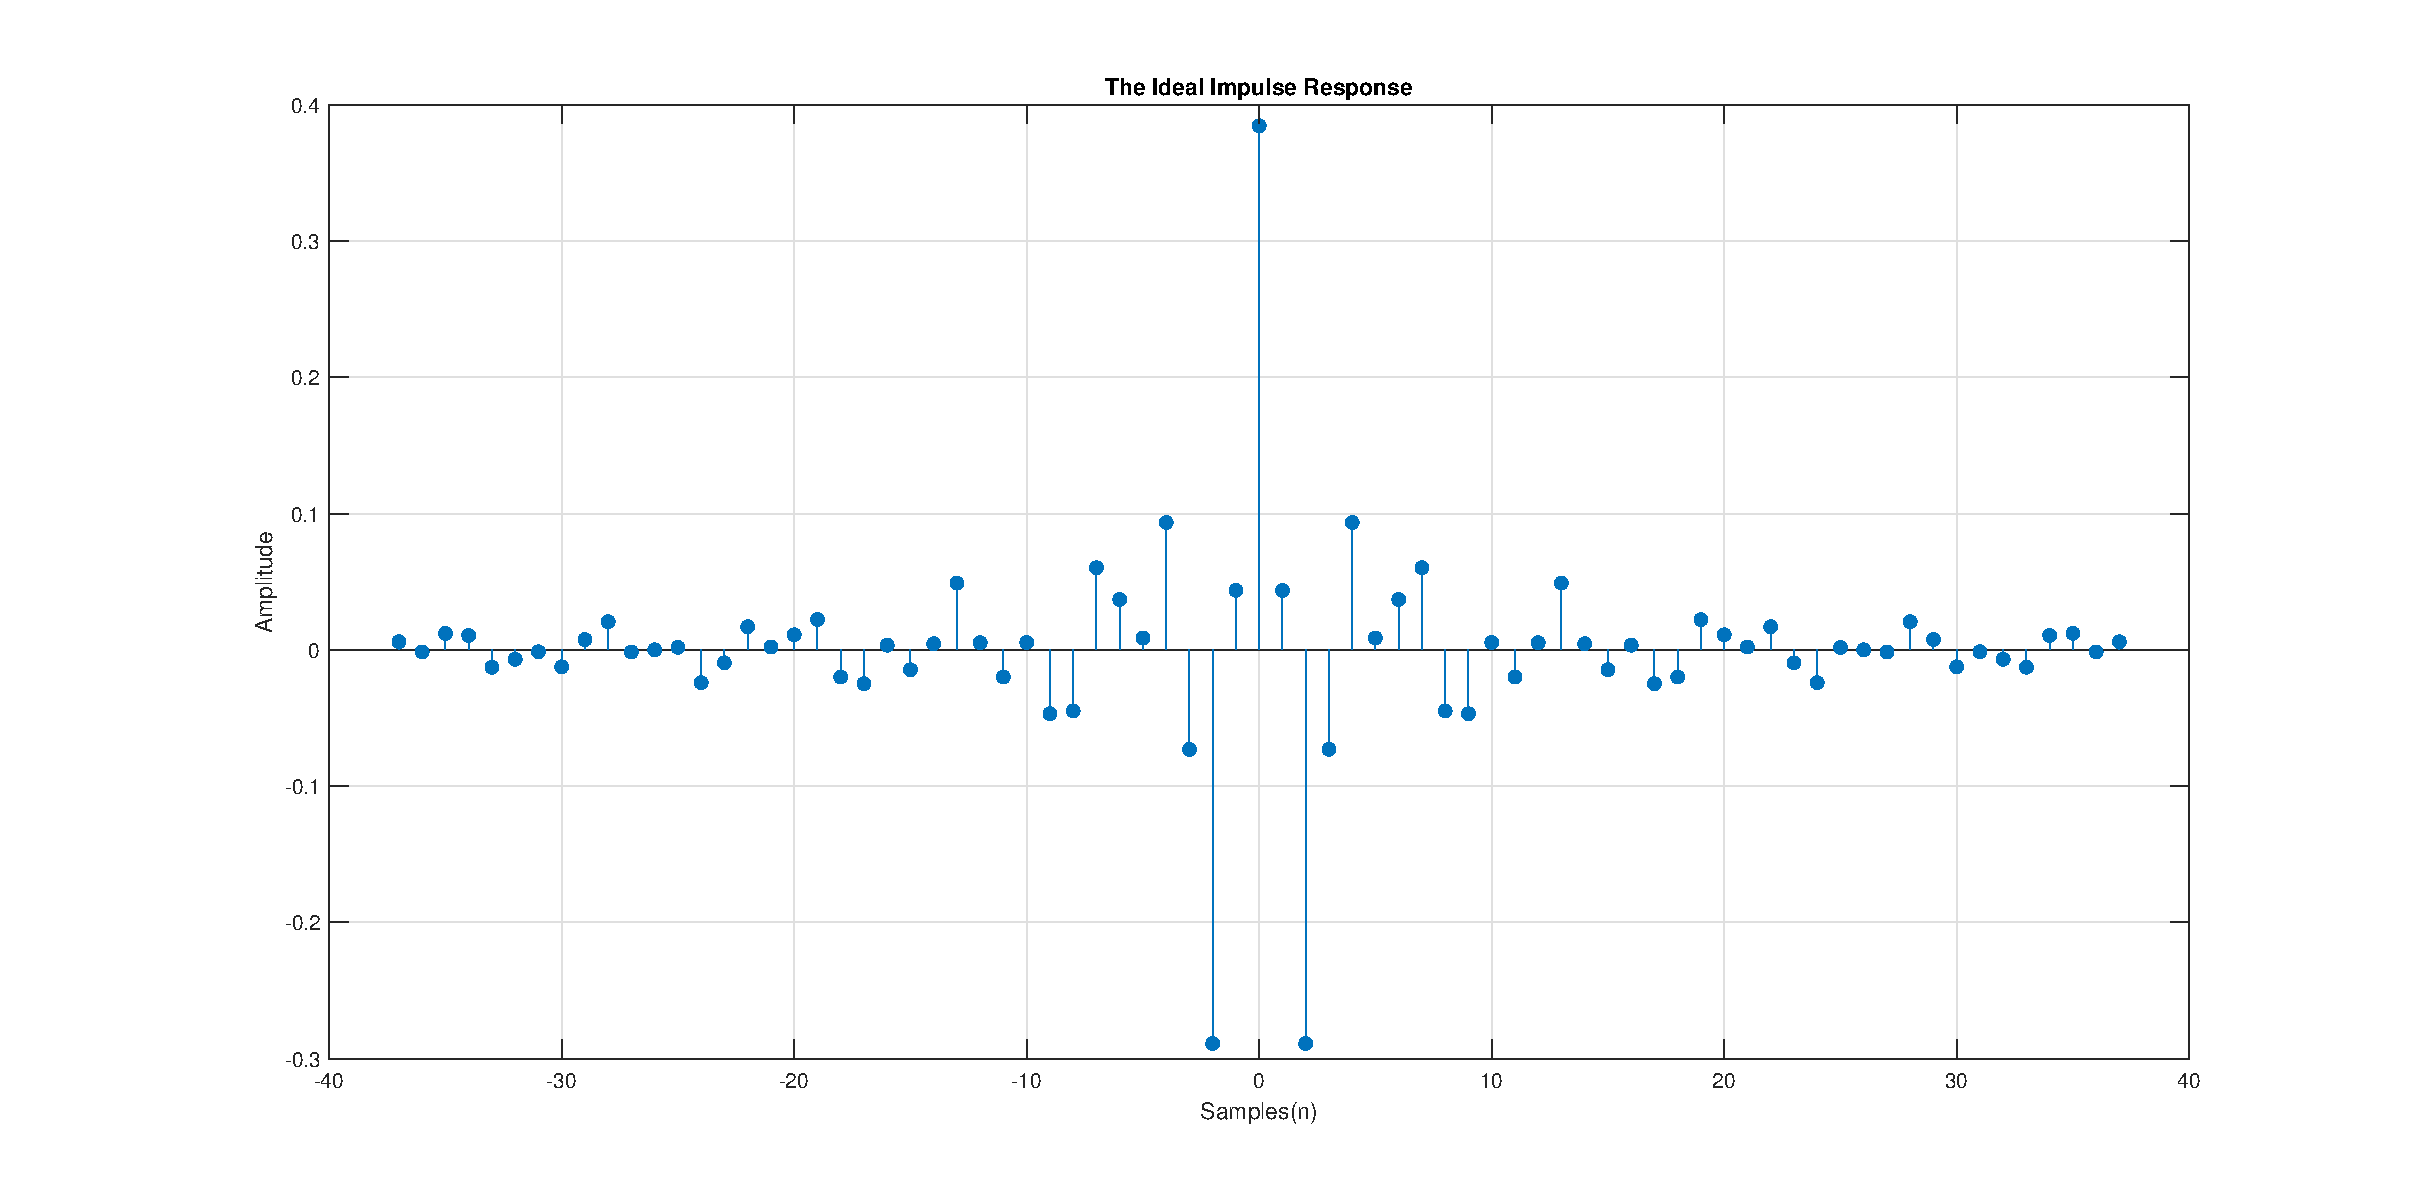
\includegraphics[scale=0.4]{figures/ideal-impulse}
	\caption{Anti-Causal Ideal Impulse Response $h_d(nT)$}
\end{figure}

\subsubsection{Truncating the Ideal Impulse Response to obtain a Finite Impulse Response}

By multiplying the ideal impulse response $h_d(nT)$ in Eq. \eqref{idealresponse} with the Kaiser window $w_K(nT)$ in Eq. \eqref{kaiser}, the ideal infinite impulse response can be truncated to obtain the finite impulse response $h(nT)$ for practical implementation.
\begin{equation}
h(nT) = 	w_K(nT).h_d(nT)
\end{equation}

\begin{figure}[!h]
	\centering
	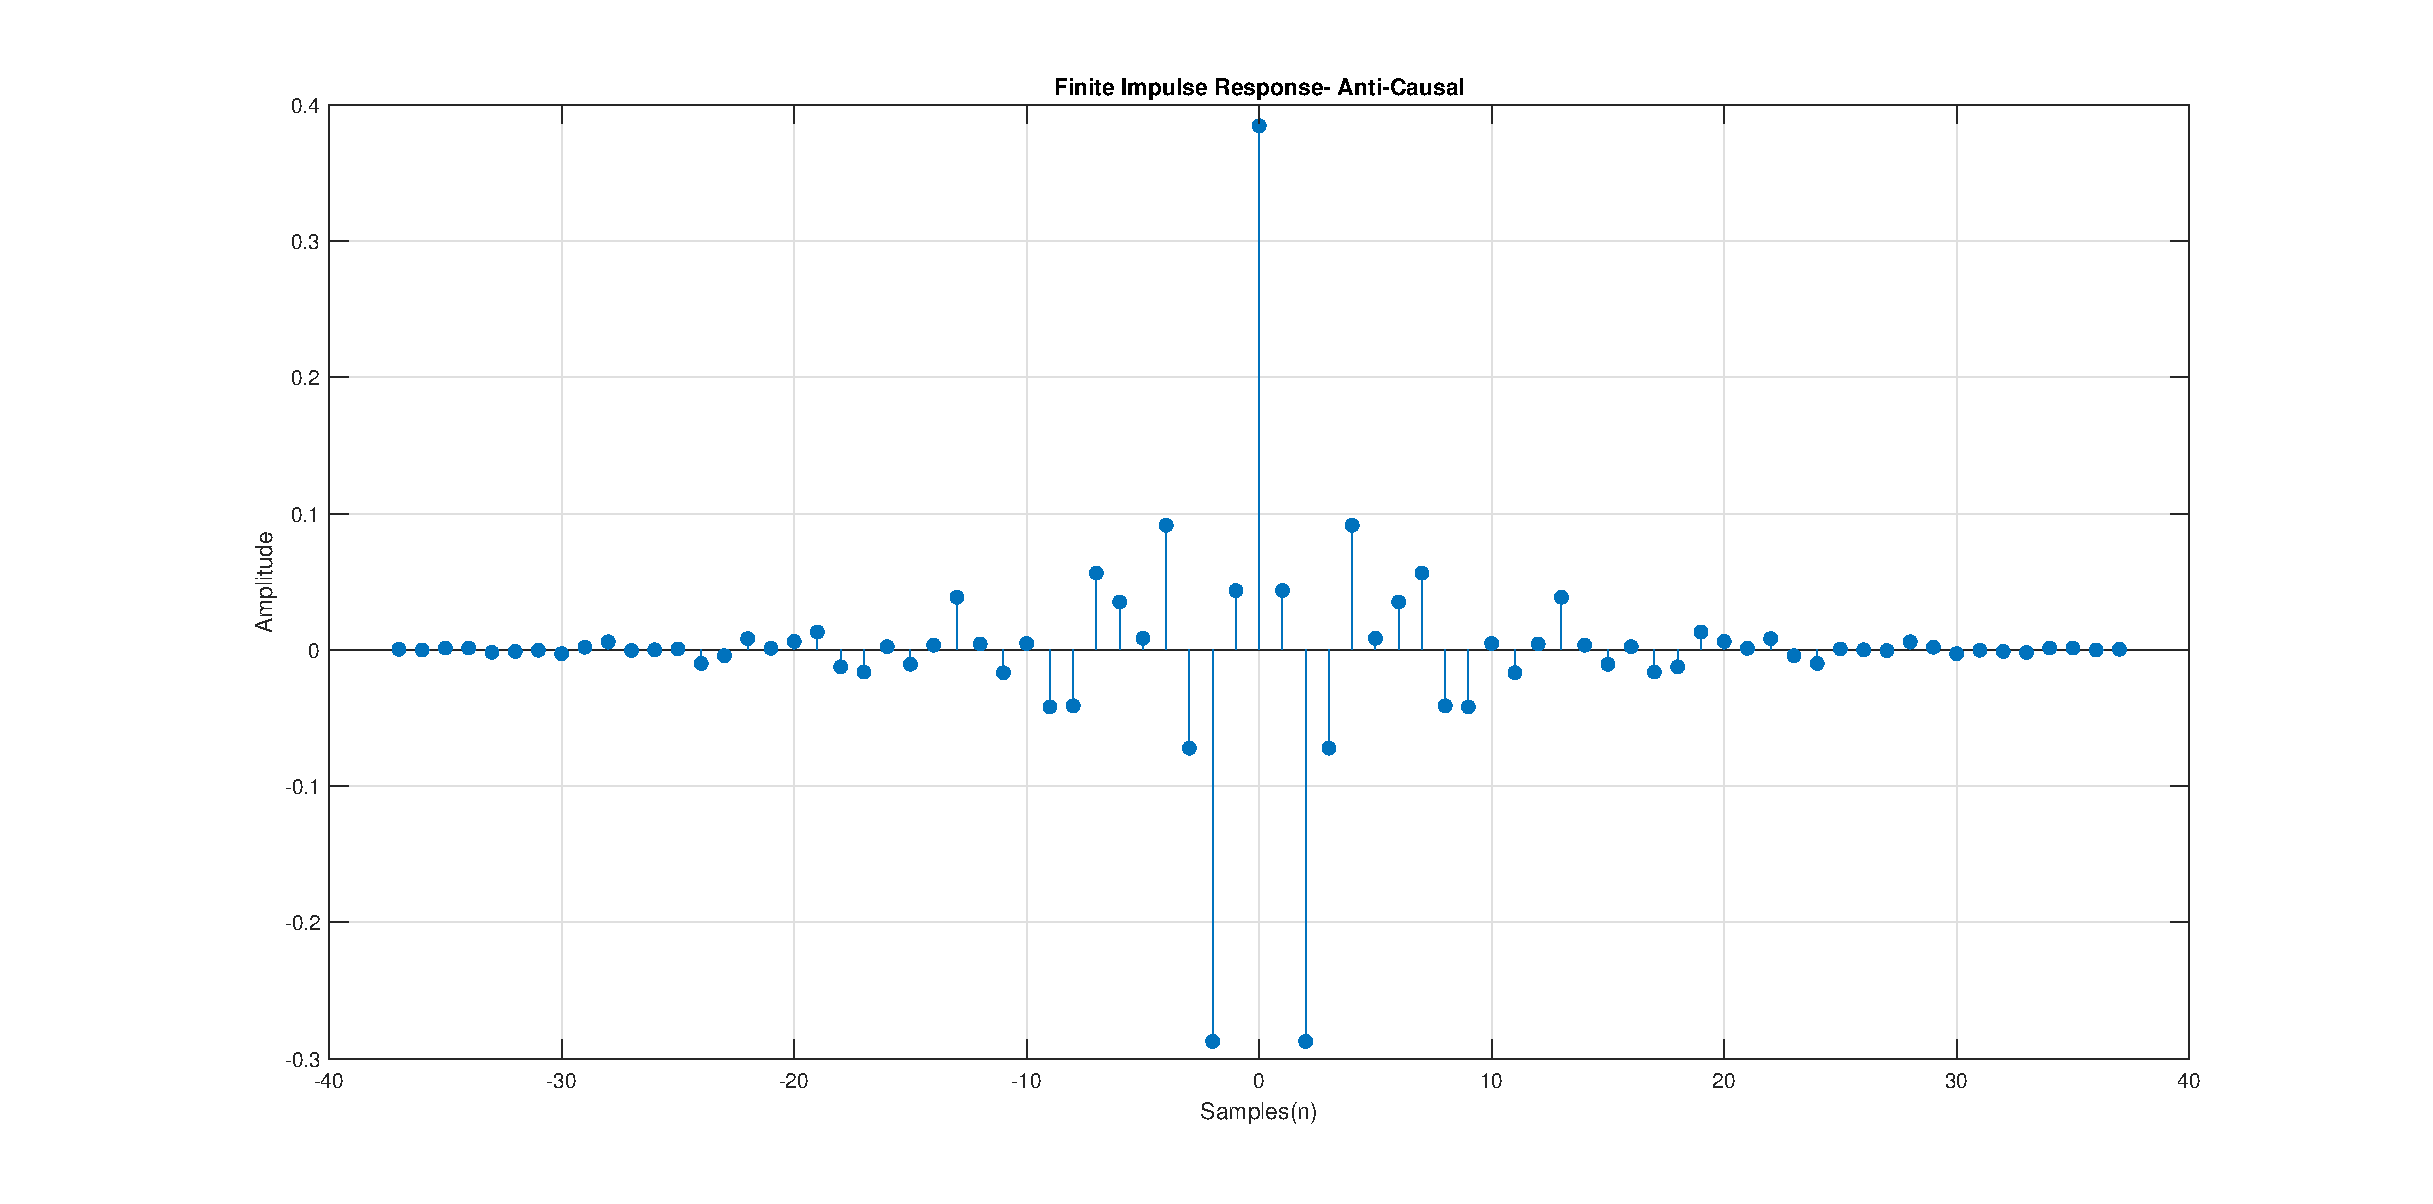
\includegraphics[scale=0.4]{figures/fir-truncated}
	\caption{Anti-Causal Finite Impulse Response $h(nT)$}
	\label{firimp}
\end{figure}

Obtaining the transfer function in the $\mathcal{Z}$ domain using $\mathcal{Z}$ Transformation,
\begin{equation}
	\begin{split}
			H'(z) &= \mathcal{Z}\left\{ h(nT) \right\}\\
		&=\mathcal{Z}\left\{ w_K(nT).h_d(nT) \right\}
	\end{split}
\end{equation}

The response is anti-causal it need to be shifted in the time domain to make it causal and get the final filter response$H(Z)$, in $\mathcal{Z}$ domain it is represented as follows. Then the equation is evaluated at $e^{j\omega}$ to get the frequency response of the filter
\begin{equation}
	H(z)= z^{-\left(\frac{N-1}{2}\right)}.H'(z)
\end{equation}

\subsection{Filter Performance Evaluation}

Performance of the filter was evaluated by using the following excitation $x(nT)$ which is a combination of three sinusoidal signals. Frequencies of these three sinusoidal signals are specified as follows to cover all three bands(\textit{lower stopband, passband and upper stopband}) in the bandpass filter.

\[x(nT) = \sum_{i=1}^{3}sin(w_inT)\]

\begin{table}[!h]
	\centering
	
	\begin{tabular}{l c c r}
		\hline
	\textbf{Parameter}& \textbf{Symbol}& \textbf{Calculation}&\textbf{Value}\\\hline
	&&&\\
	Middle frequency of the lower stopband& $\omega_1$&$\frac{0+ \omega_{a1}}{2}$&125 rad/s\\
	Middle frequency of the passband &$\omega_2$&$\frac{\omega_{p1}+\omega_{p2}}{2}$&600 rad/s\\
	Middle frequency of the upper stopband& $\omega_3$&$\frac{\omega_{a2}+\omega_s/2}{2}$&1100 rad/s\\
	\hline\hline
	\end{tabular}
\caption{Frequencies for Filter Performance Evaluation}
\end{table}

The required filtered output can be obtained by time domain convolution of the input signal $x(nT)$ with the impulse response $h(nT)$ in Fig. \ref{firimp}. But as mentioned previously the convolution is computationally expensive operation. Therefore filtering is done in the frequency domain which then simplifies into a simple multiplication. For that Discrete Fourier Transform(DFT) of the input signal $x(nT)$ and DFT of $h(nT)$ are obtained through the {\tt fft()} function in MATLAB. Then they are multiplied to get the frequency domain output and {\tt ifft()} is applied on that to get the time domain output signal.
 
\begin{figure}[!h]
	\centering
	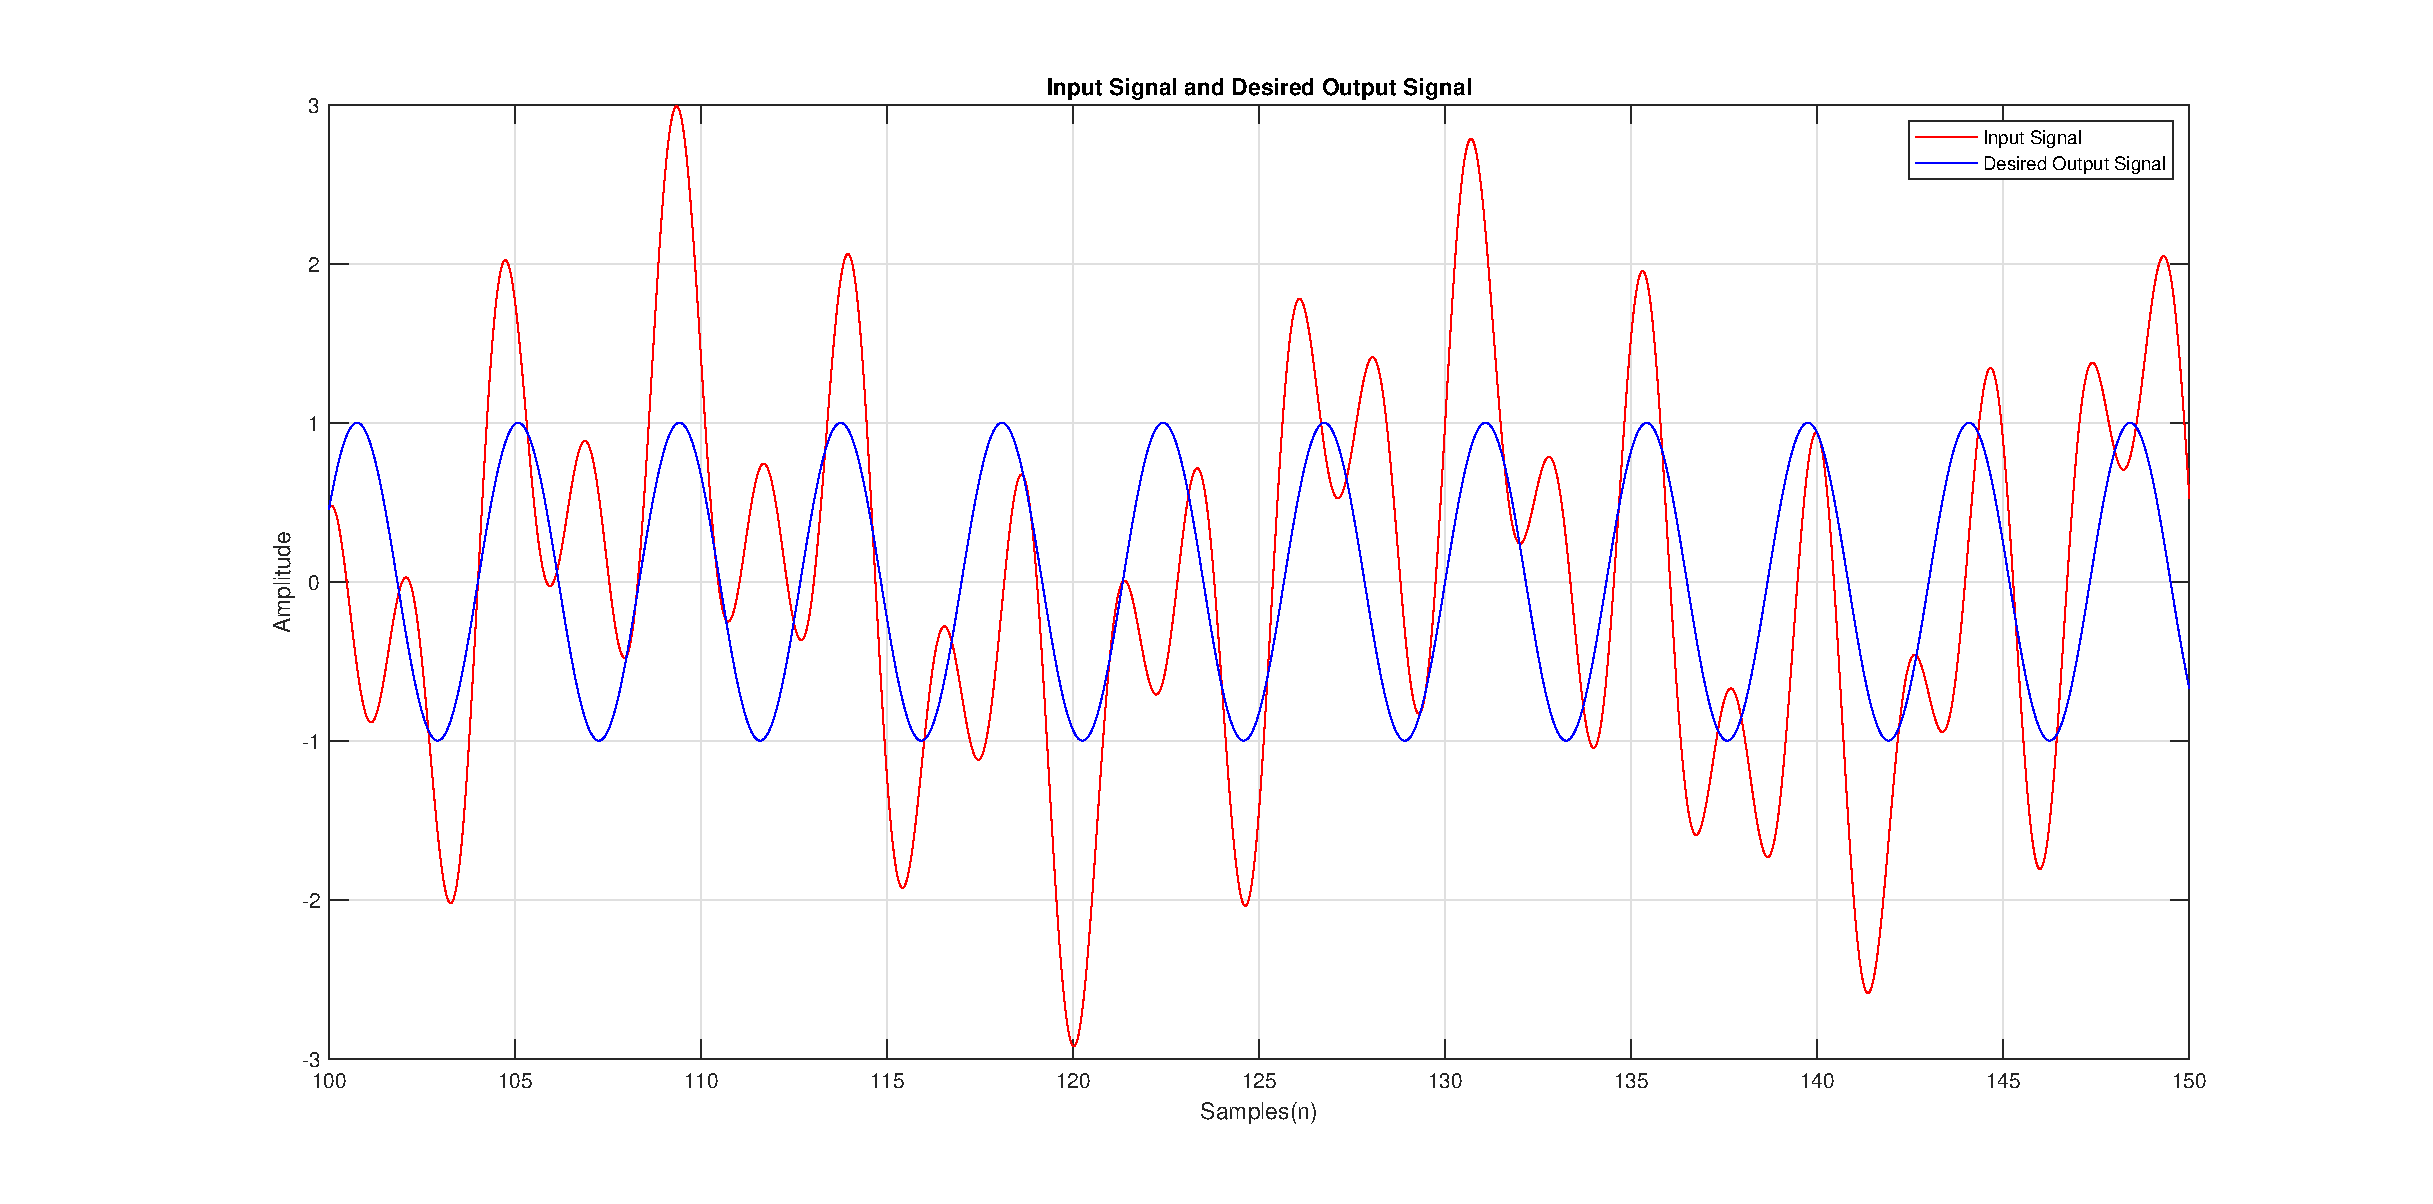
\includegraphics[scale=0.4]{figures/in-signal}
	\caption{Input Signal and the Desired Output Signal}
\end{figure}

\pagebreak
\section{Results}

\subsection{FIR Filter Characteristics}

Filter Characteristics showed in this section was obtained through the procedure explained in the \textit{section 2.1 Filter Implementation}.\\

Anti-Causal Impulse Response of the Filter can be right shifted in time domain to obtain the Causal Impulse Response as shown below. Note that there, the samples(n) axis starts from 0 and continues up to 74. That is N-1. Whereas previously it was from -37 to 37.

\begin{figure}[!h]
	\centering
	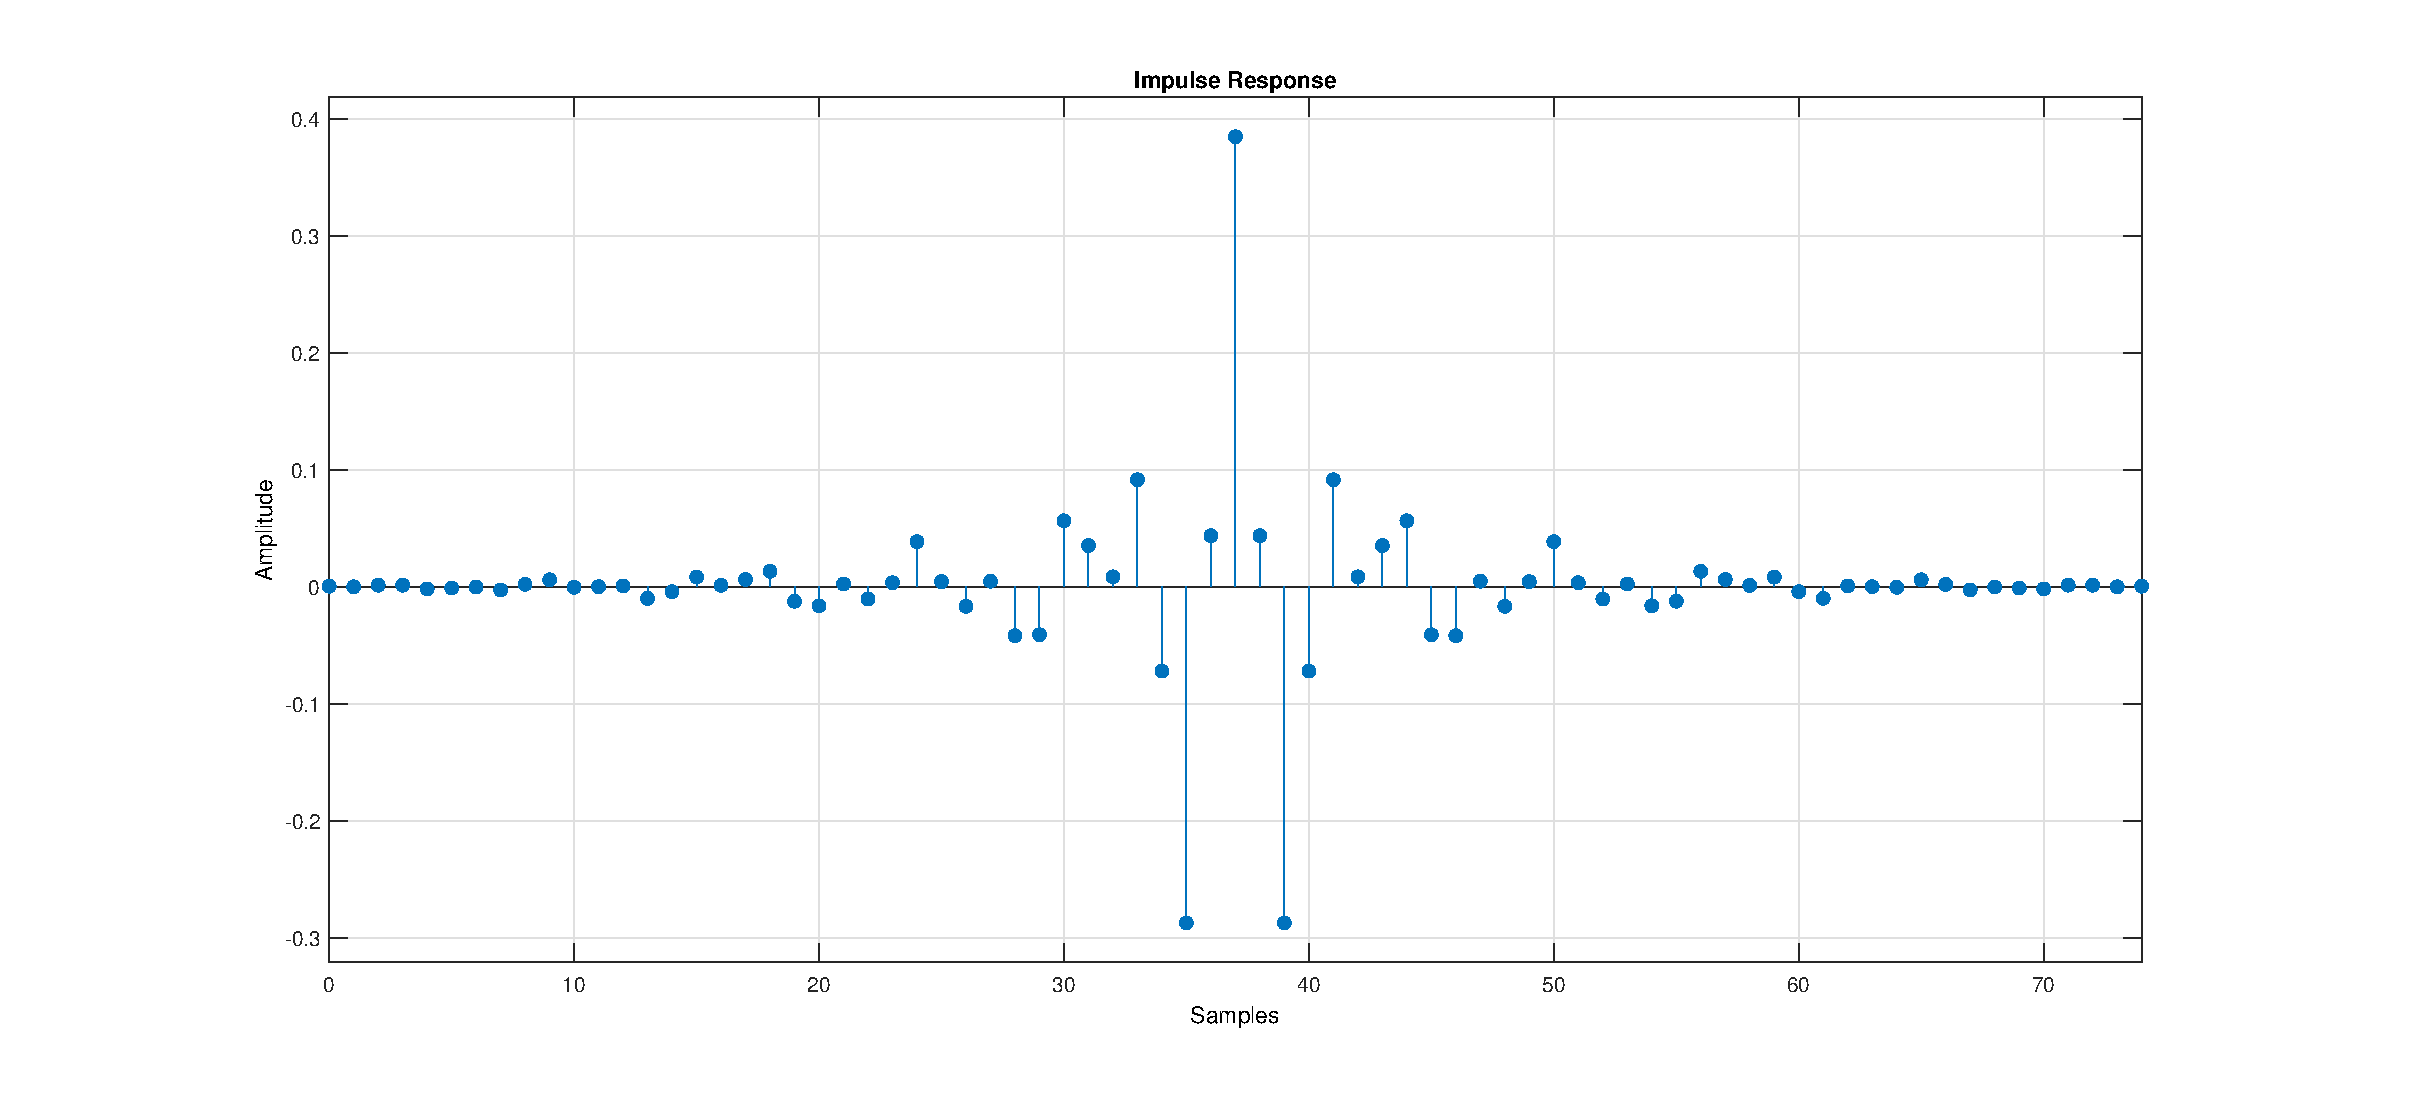
\includegraphics[scale=0.4]{figures/causal-impulse-response}
	\caption{Causal Impulse Response of the Filter}
\end{figure}
\vfill
Magnitude Response of the Filter was obtained through the MATLAB's {\tt freqz()} function which computes the frequency, magnitude, and phase response of given digital filter(\textit{impulse response}).
\begin{figure}[!h]
	\centering
	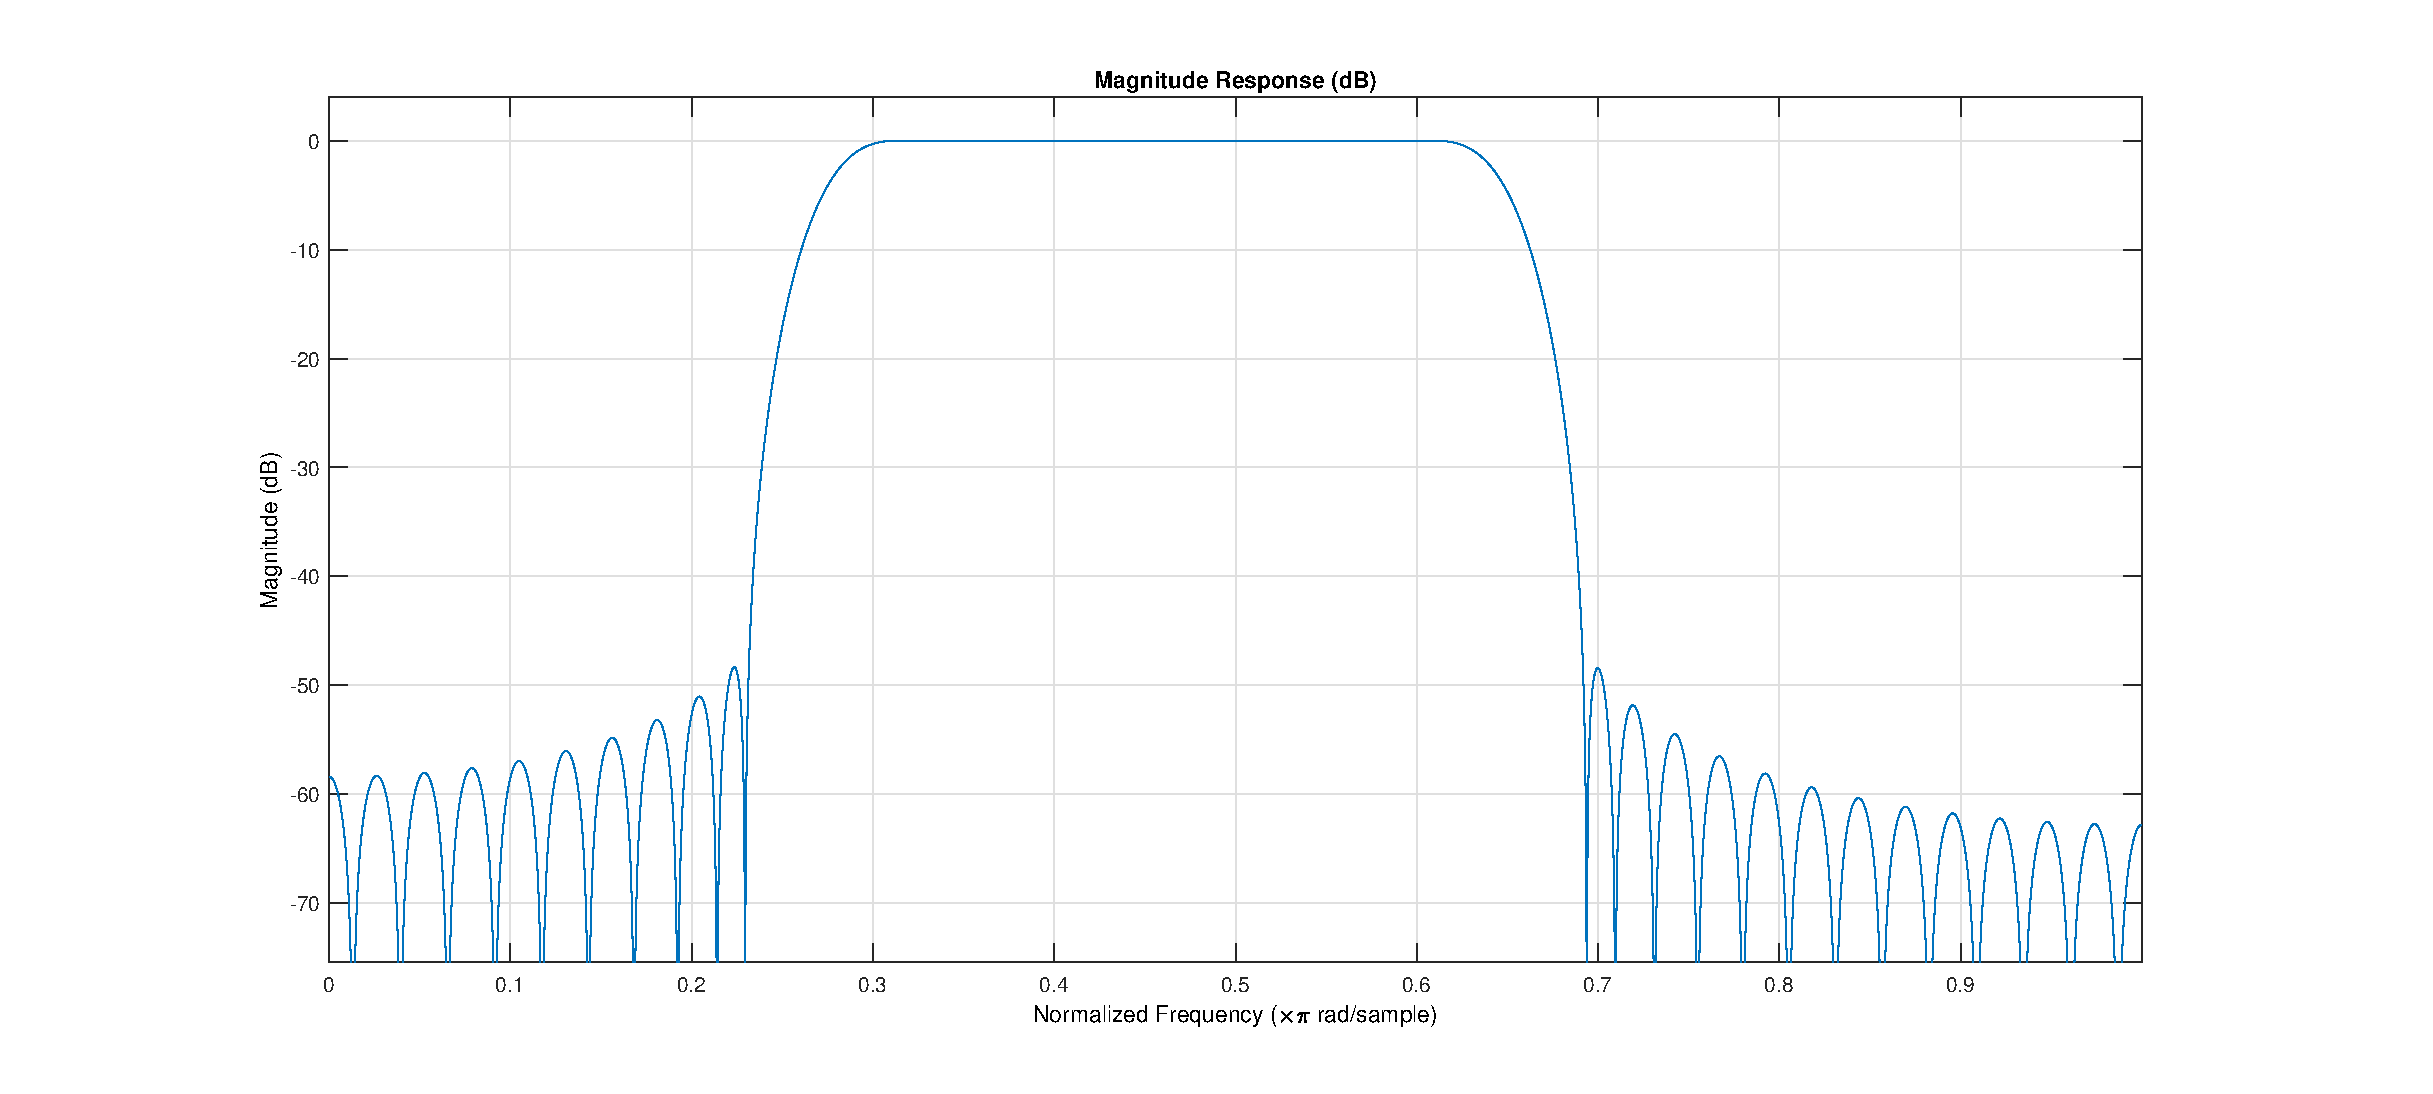
\includegraphics[scale=0.4]{figures/magnitude-response}
	\caption{Magnitude Response of the Filter}
\end{figure}

\pagebreak
Magnitude Response of the Filter for the frequencies in the Passband can be simply obtained through limiting the range of Angular Frequency axis using MATLAB's {\tt xlim([$\omega_{p1}$ $\omega_{p2}$])} function. It allows us to identify the nature of the passband  ripples of a kaiser window of order 75. According to the prescribed specifications Maximum passband ripple(\textit{desired})  $\tilde{A_p}$ was 0.09 dB. And we can observe that the designed filter has achieved that goal.

\begin{figure}[!h]
	\centering
	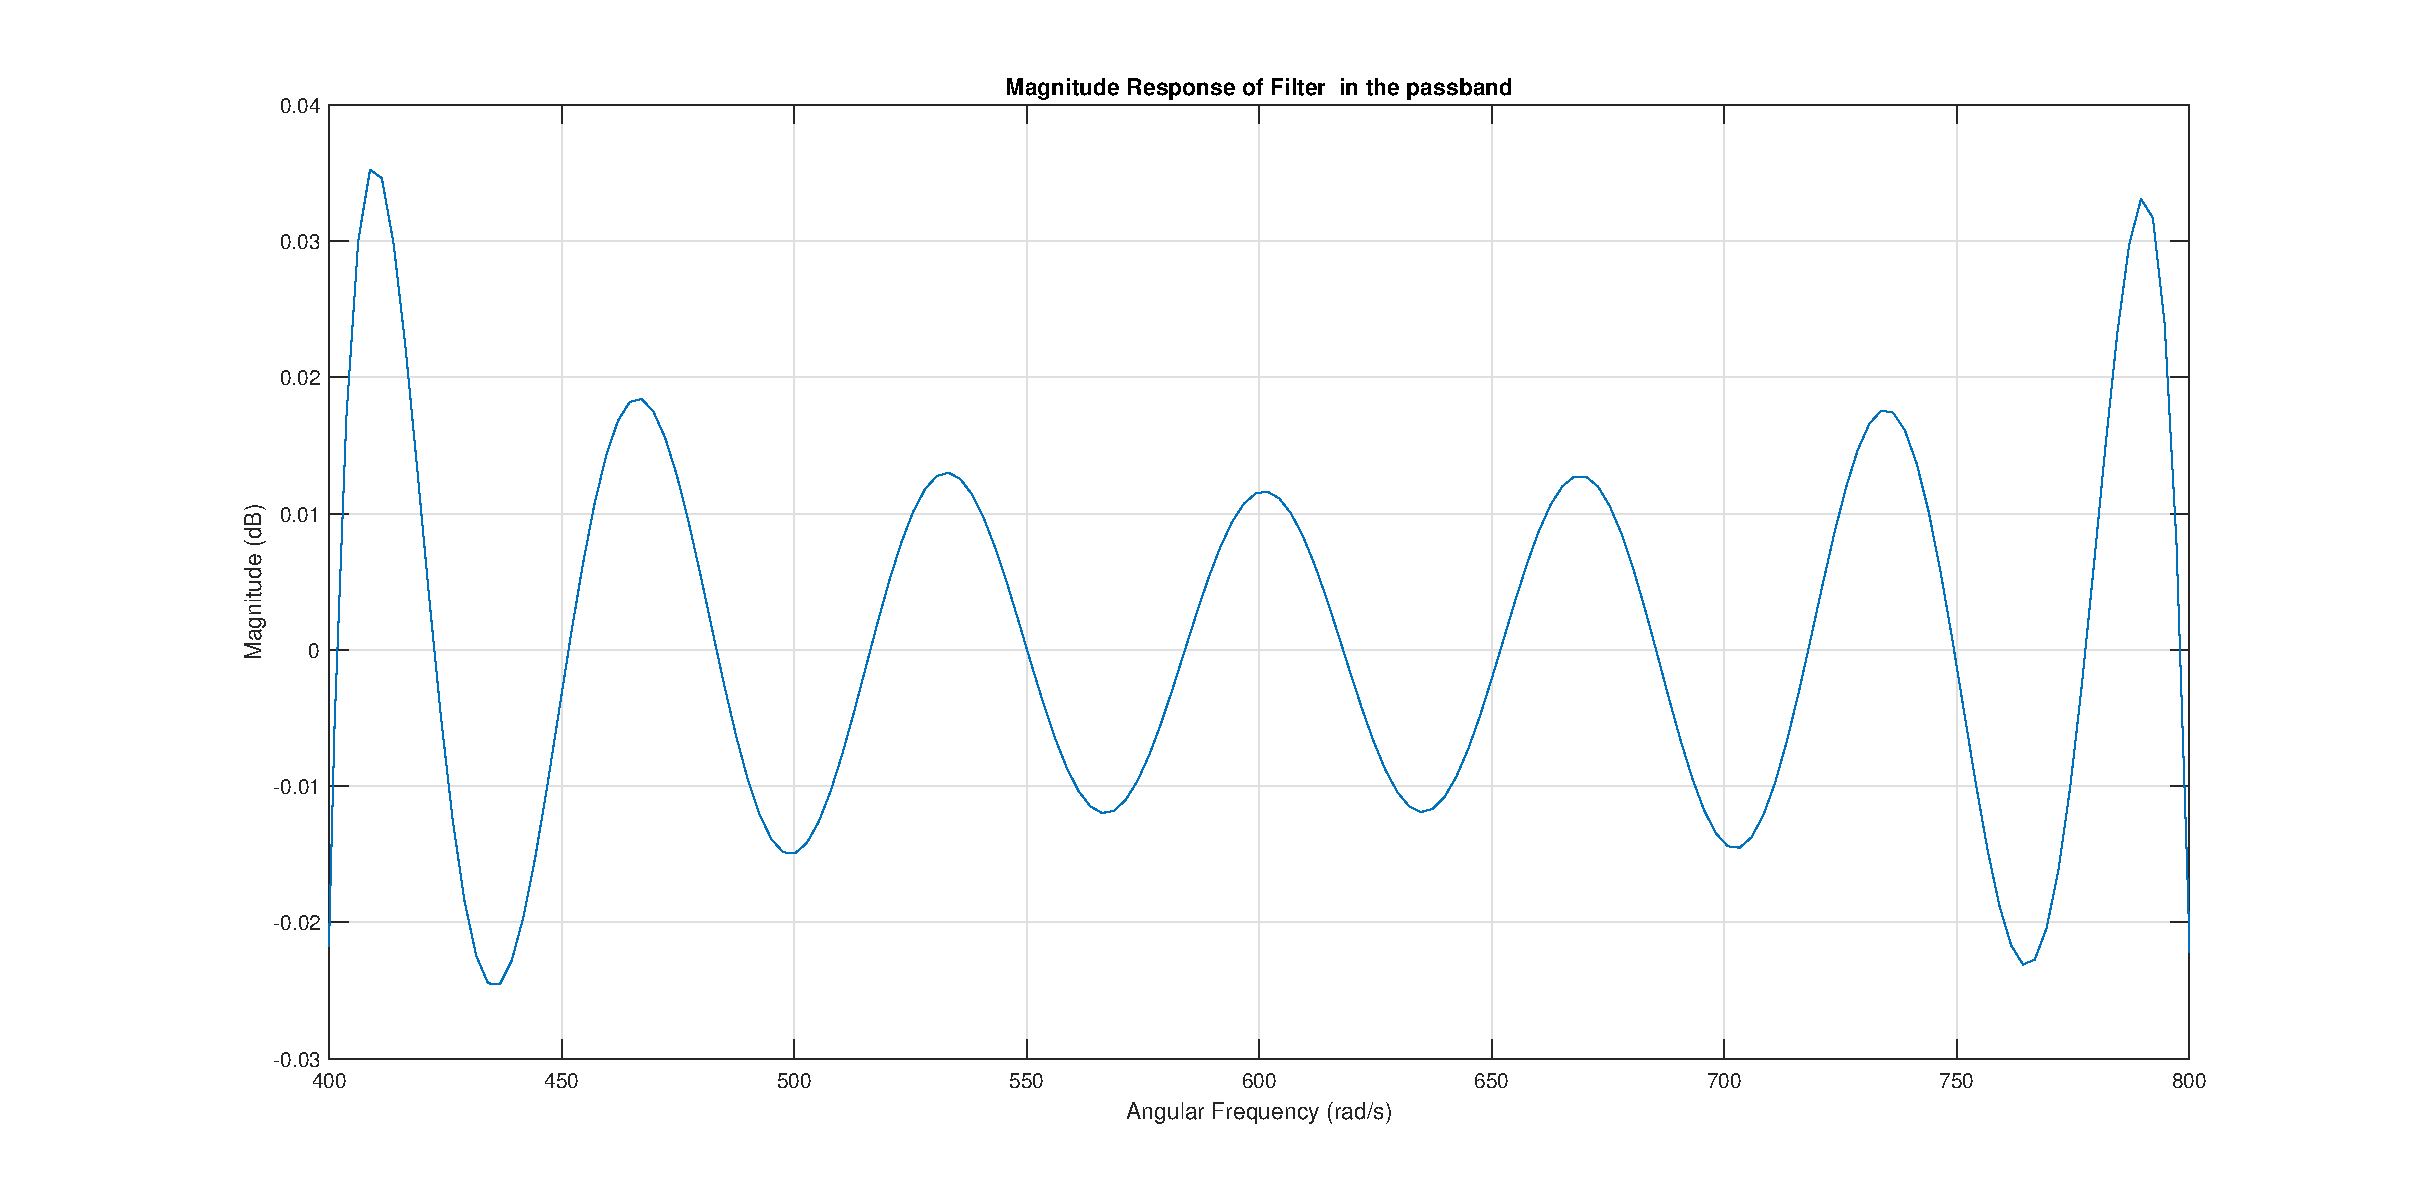
\includegraphics[scale=0.4]{figures/magnitude-resp-passband}
	\caption{Magnitude Response of the Filter for the frequencies in the Passband}
\end{figure}

\pagebreak
\subsection{Input Output Signal Characteristics}

As explained in the \textbf{Filter Performance Evaluation} section input signal is a combination of three sinusoidal signals which has its frequency components lie in the three bands of the bandpass filter. This fact is clearly visible in the frequency spectrum of the Input Signal.

\begin{figure}[!h]
	\centering
	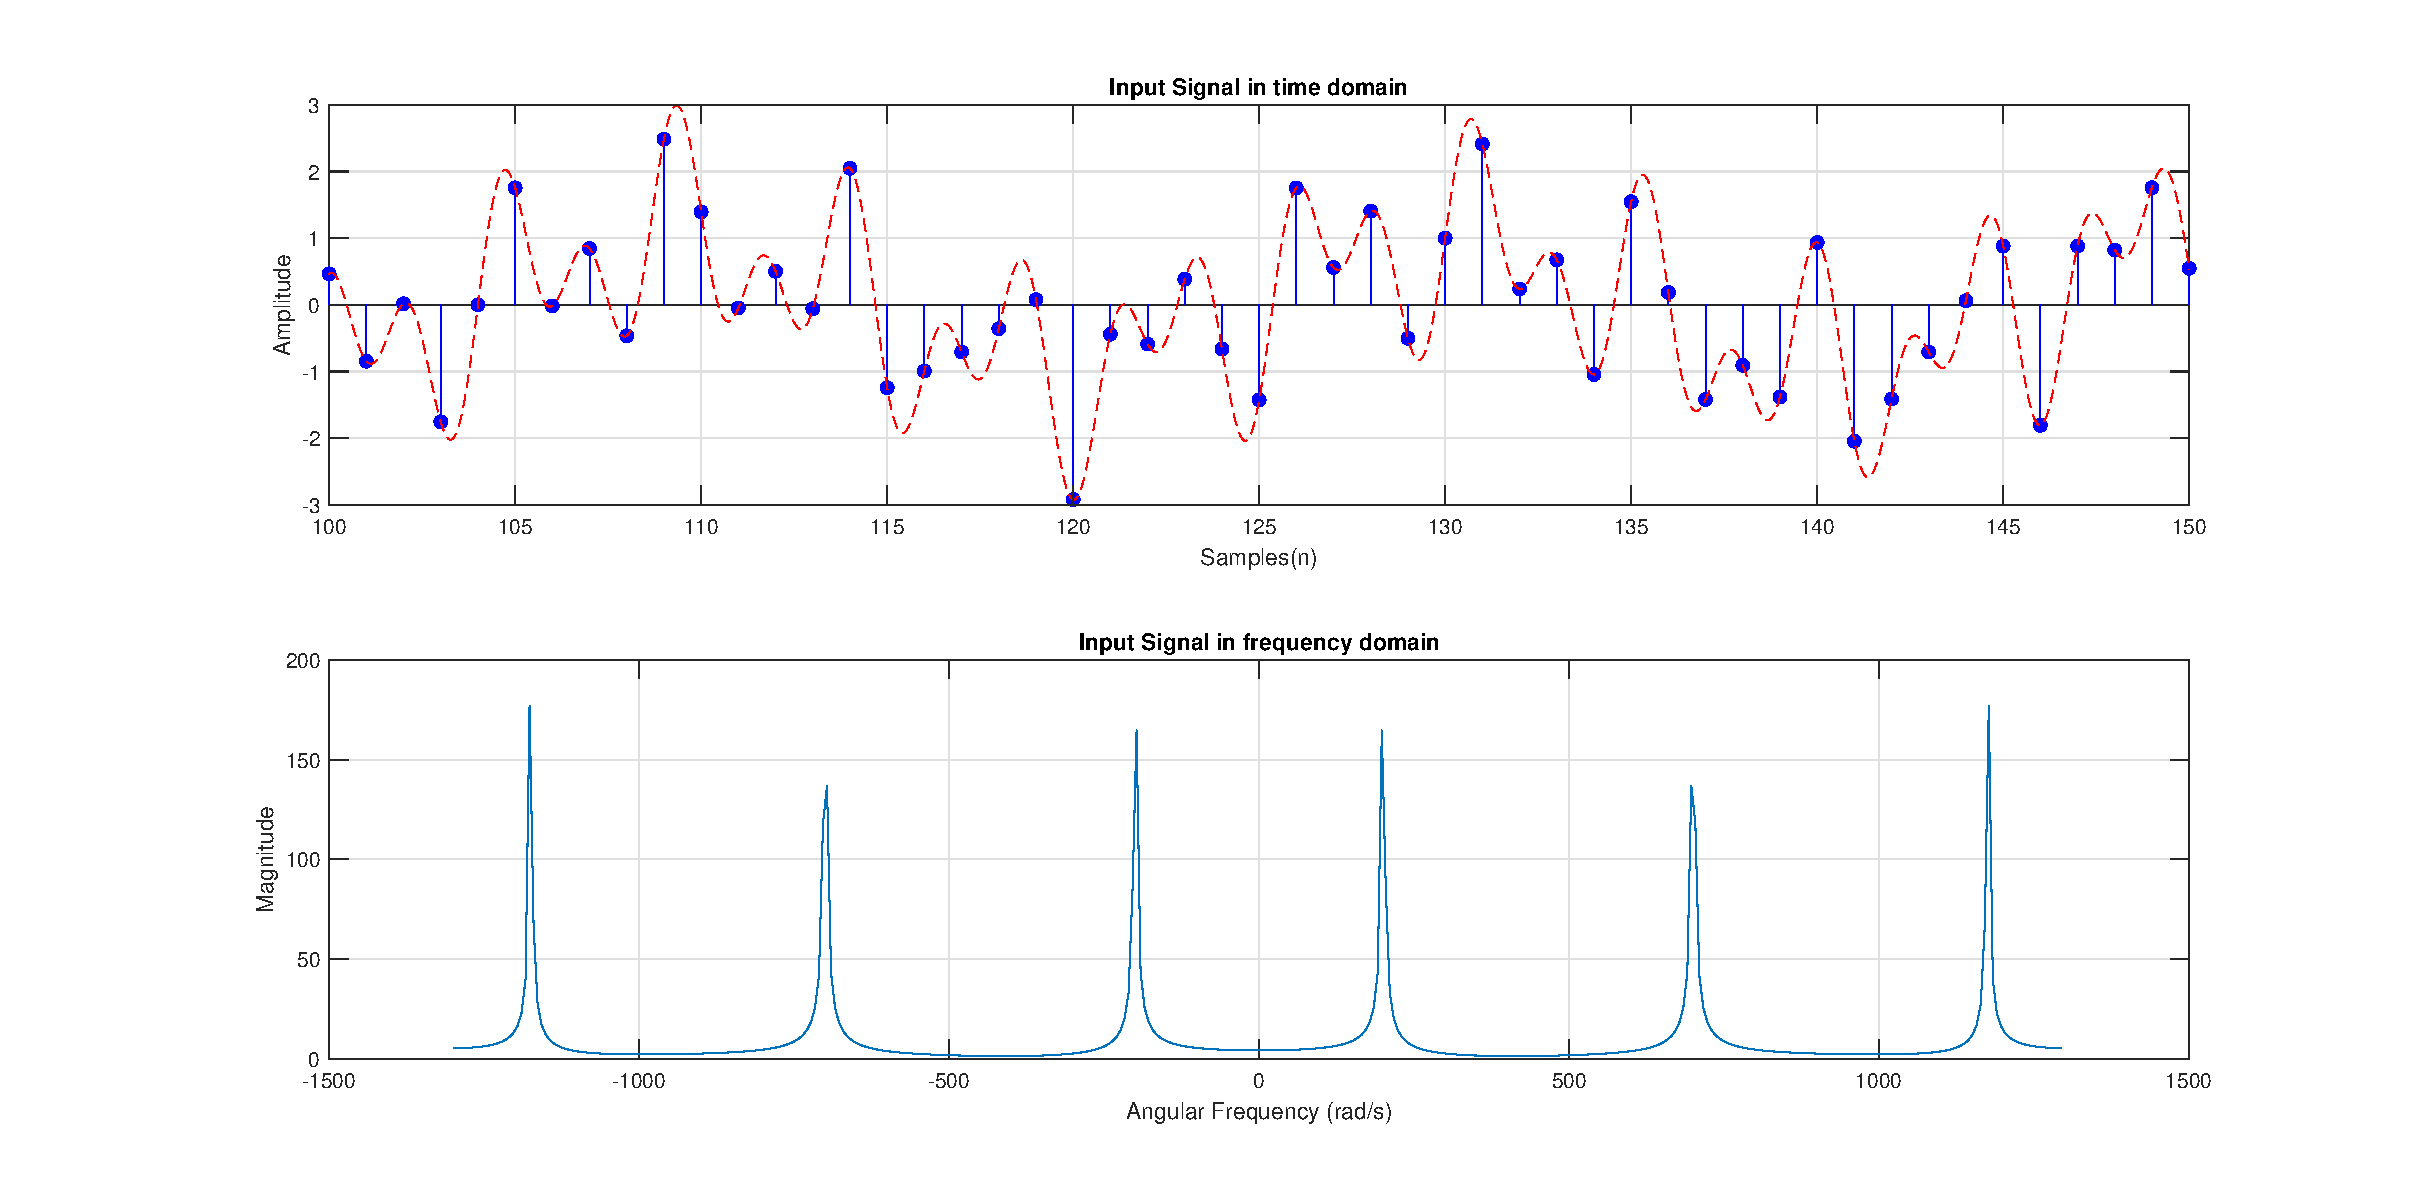
\includegraphics[scale=0.45]{figures/input-signal}
	\caption{Input signal representation in Time and Frequency Domains}
\end{figure}
\vfill
By inspecting the frequency spectrum of the output signal we can observe that output signal is a filtered version of the input signal and that the correct frequencies have been passed through the filter perfectly. Because both the frequencies that were in the lower and upper stop bands are filtered out and disappeared completely from the frequency spectrum of the output signal. This guarantees that the Kaiser window method has  yield an almost ideal bandpass filter which satisfies the prescribed specifications.

\begin{figure}[!h]
	\centering
	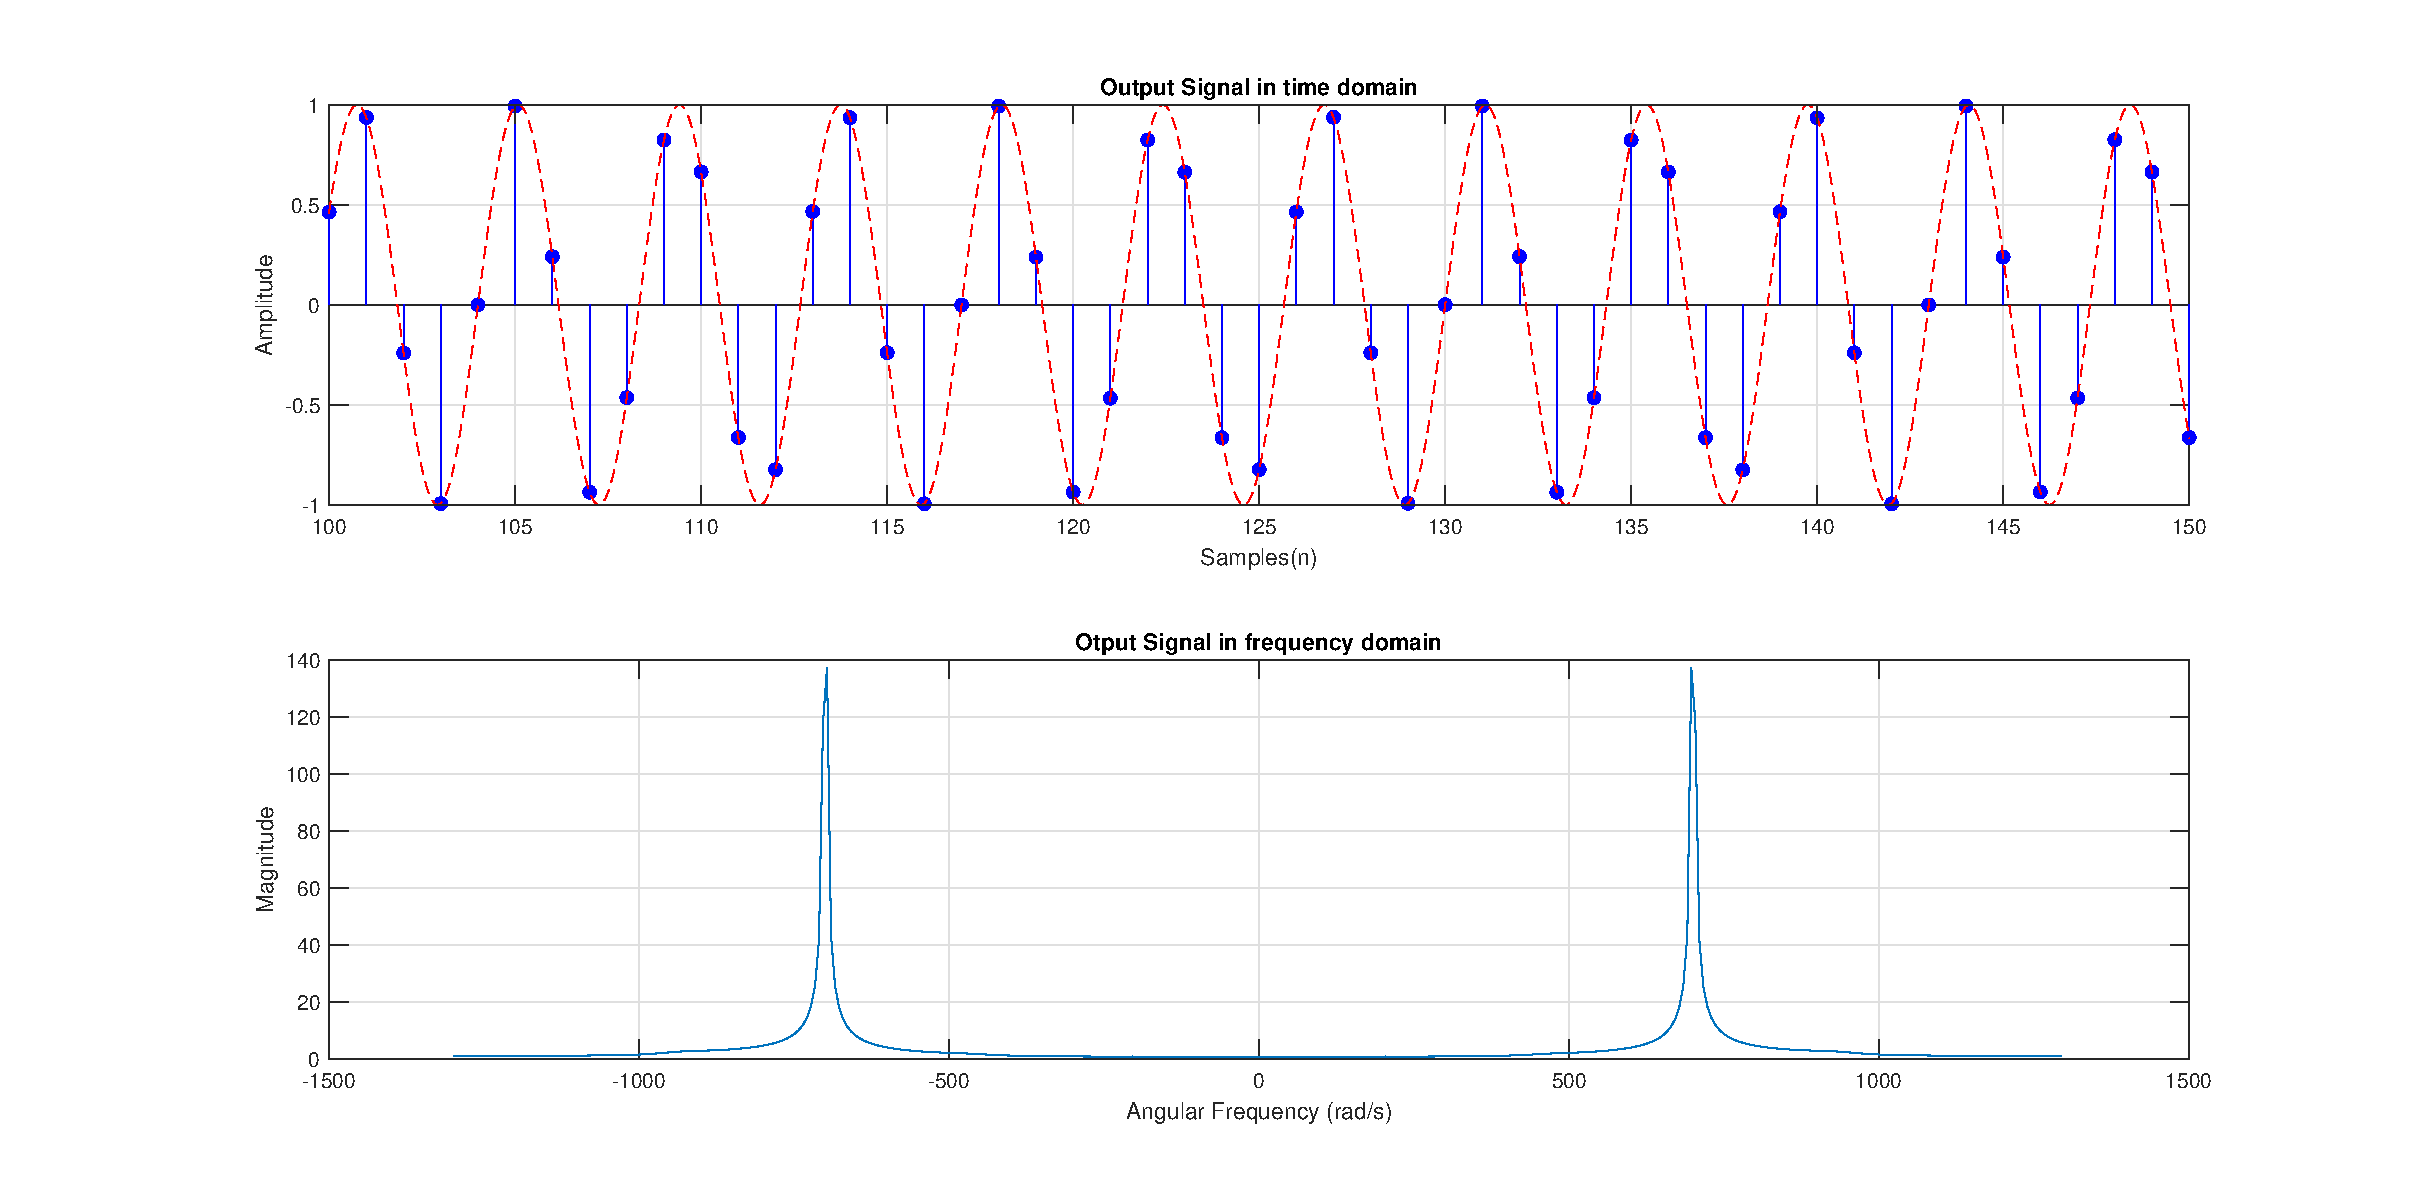
\includegraphics[scale=0.45]{figures/output-signal}
	\caption{Output signal representation in Time and Frequency Domains}
\end{figure}
\pagebreak

\section{Conclusions}

Depending on the results it can be concluded that the Kaiser Window method has yielded a near ideal passband filter characteristics which satisfies all the prescribed specifications. Even though there are some ripples in the passband and the stopband, the filter characteristics can be optimized without much effort through tuning the parameters ($\alpha$ and $N$) to obtain perfect and at the same time practical filter for a given application. In addition to that computational complexity of the parameters which are used to obtain the Kaiser Window is also much less and most importantly there is a clear method to obtain those parameters through empirical formulae.\\

But when a filter is practically implemented in hardware, usage of the computational resources plays a vital role and as the order of the filter grows resource requirement grows drastically. Therefore,  as a major disadvantage of the Kaiser Window method, the high order of the filters can be pointed out. Filter of order 75 was required to achieve the given specs in our case while there are other filter designing methods which yield the same characteristics with much lower order and therefore much lower resource requirements.

\vfill
\hrule
\vspace{0.5cm}
\bibliographystyle{plain}
\bibliography{refer}


\vspace{1cm}
\hrule
\vspace{0.5cm}
\begin{appendices}
	\section{Matlab Code for the Implementation}
	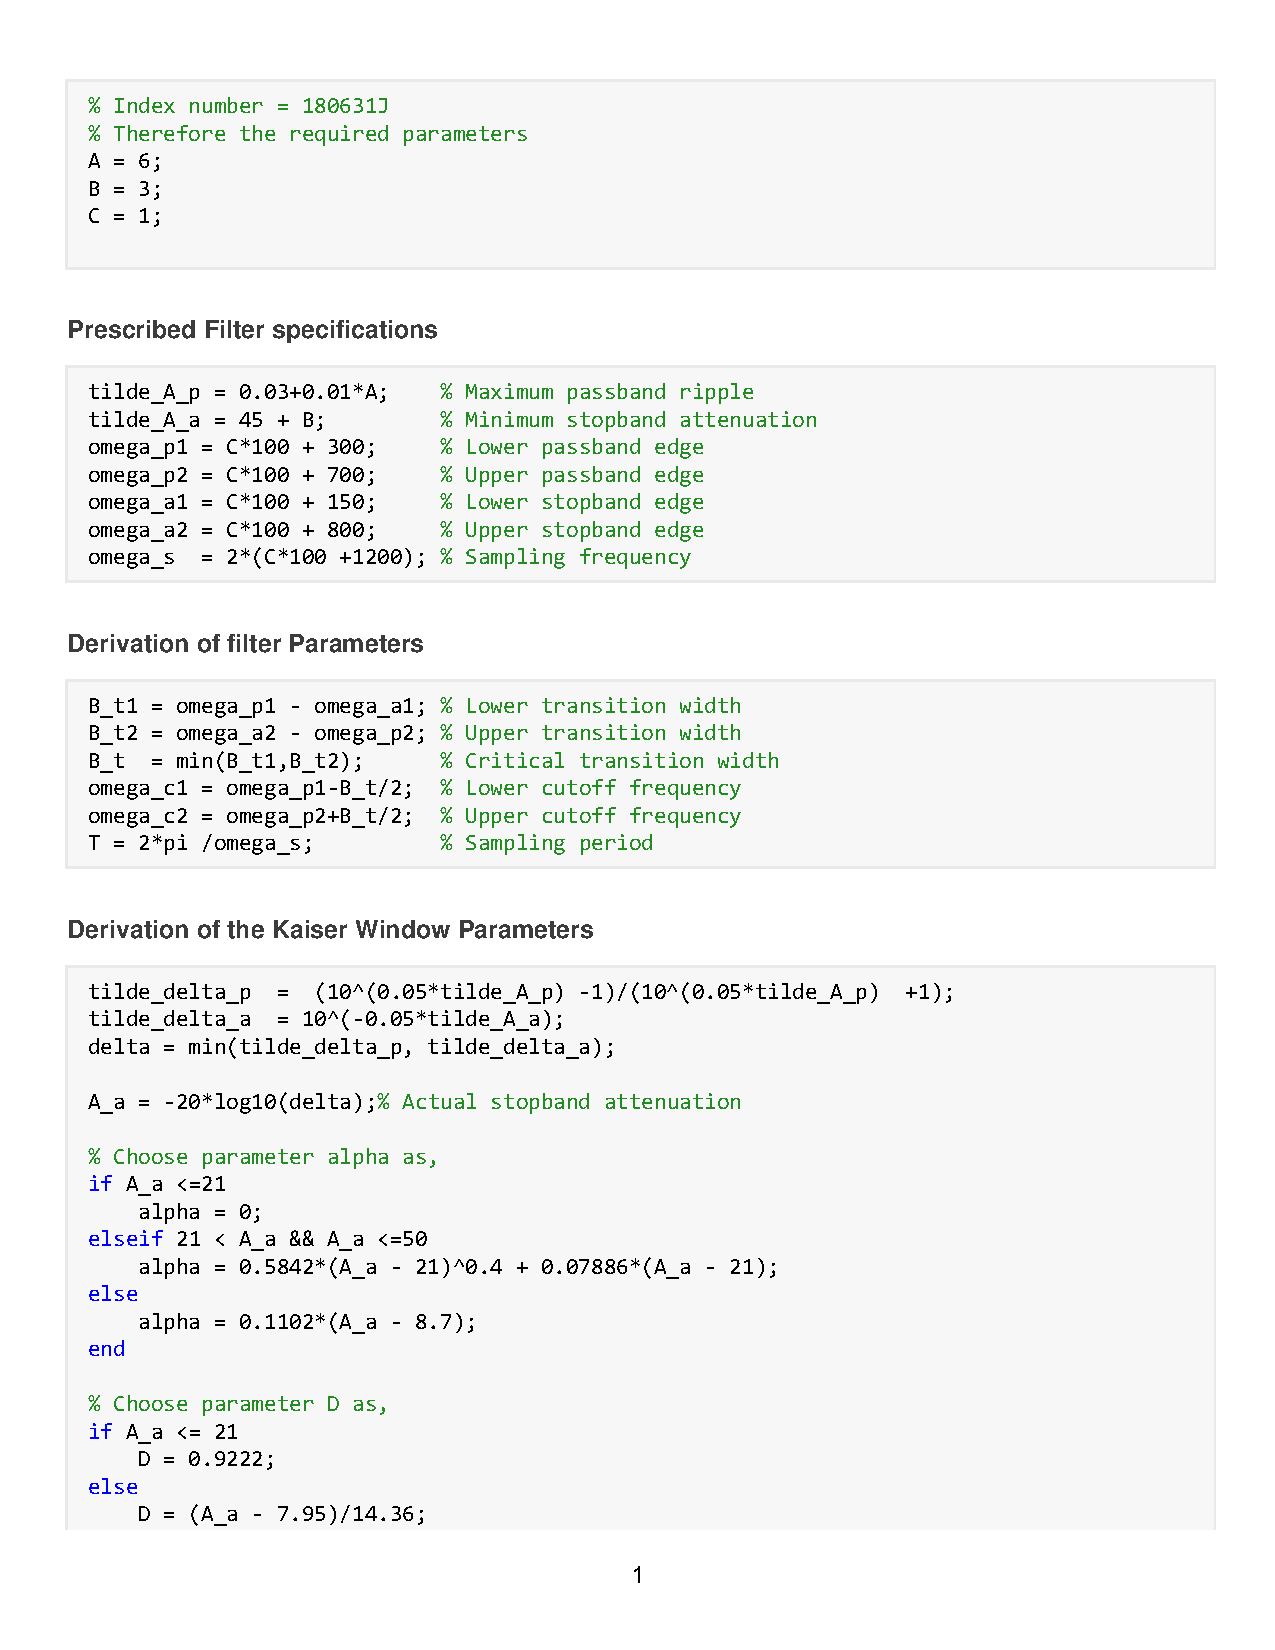
\includepdf[pages=-]{code/bandpass180631J.pdf}
\end{appendices}



%---------------------------------------------------------------------------
\end{document}
-
